\section{掌握CUDA GPU并行编程（硬件与软件）Nsight Compute入门}

本章本来应该开始讲解如何使用 Nsight Compute 工具来分析 CUDA 应用。然而开始着手做这件事时，发现了一个可能遇到的问题，尤其是使用 Windows 操作系统的话，下面解释这个问题及其解决方案。

\subsection{问题分析：ncu工具报错}

首先这是 CUDA 课程文件夹，使用 \texttt{ls} 命令来列出所有文件和文件夹。如所示，有一些 CUDA 文件，还有一些可执行文件，接下来执行这个应用——向量加法项目的可执行文件。前文已经解释过很多次了，如所示，它正确执行没有任何问题，执行时间等于 6.8 毫秒。然而当开始分析这个应用时：

如果想使用 Nsight Compute 进行分析，需要输入 \texttt{ncu}，它指的是 Nsight Compute。点击回车看看输出。如所示，有一些错误，这是第一个。此外，还有另外三个错误。

为什么 Nsight Compute 工具不工作呢？它安装在系统里了吗？答案是肯定的。当安装 CUDA 工具包时，安装了许多库和工具，其中之一就是 Nsight Compute，但这不是遇到的错误。除非在这里遇到错误说 \texttt{ncu} 命令未找到，否则不需要安装 Nsight Compute。

\begin{figure}
    \centering
    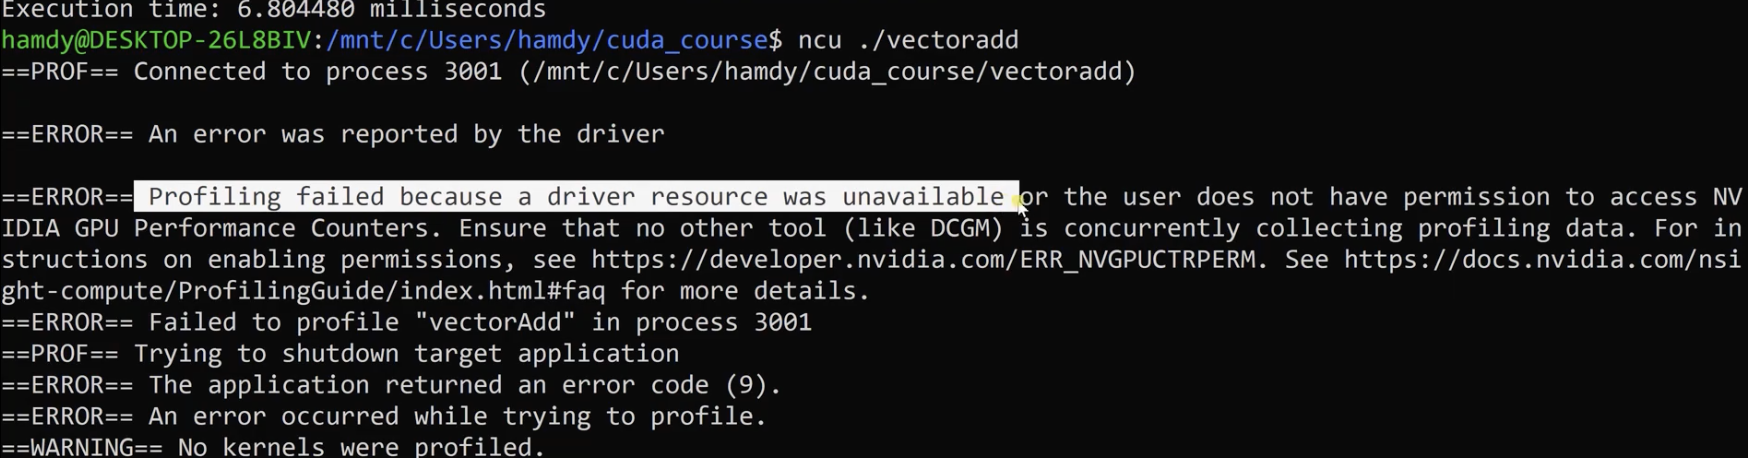
\includegraphics[width=0.75\linewidth]{resources/cuda-097.png}
    \caption{}
    \label{fig:placeholder}
\end{figure}

\subsection{GPU性能计数器权限设置}

现在检查一下这五个错误中的每一个。第一个提到驱动程序有问题，还记得这个吗？如何检查驱动程序呢？前文在解释 \texttt{nvidia-smi} 工具时提到过驱动程序。输入这个命令，看看驱动程序是否已安装。这个表格不会在这里出现。如果驱动程序有问题，这个表格将不会显示。

会遇到一个问题或错误，类似这里的情况。如所示，这里提到了驱动程序版本，甚至还有 CUDA 版本，以及 NVIDIA GeForce RTX 3090 GPU 被检测到了，驱动程序版本被检测到了，CUDA 版本被检测到了，这不是问题所在。如果这不是问题，为什么错误提到有驱动程序问题呢？这可以从第二个错误中理解。如果阅读第二个错误，就会找到答案。它说分析失败，因为一个驱动程序资源不可用，"或者"解答了问题，"或"意味着这可能是个问题，也可能不是。

那么现在检查的问题不是第一个。检查问题是否在这个部分。它说用户没有访问 GPU 性能计数器的权限。需要搜索关于 GPU 性能计数器限制的信息，以获得更多信息。下面给出解决方案：在 Windows 系统上安装 GPU 驱动程序时，它只将 GPU 性能计数器的访问权限授予管理员，而当前不是以管理员身份运行，是以普通用户身份运行。

可能会问为什么不用 sudo？因为使用 sudo 时，如所示，可能会遇到另一个问题——\texttt{ncu} 命令未找到。但确定已经安装了 Nsight Compute 工具，接下来尝试搜索 NVIDIA 面板。

如所示，右键点击并选择 NVIDIA 控制面板选项，需要几秒钟来打开一个窗口。从这个窗口，需要进入菜单并选择桌面。然后从桌面启用开发者设置，启用这个选项，将在这里显示性能计数器。请看这一部分启用。

如所示，有了开发者设置管理 GPU 性能计数器其中之一，也是这里唯一可用的。点击这里，如所示，有两个选项。第一个是仅限管理员用户访问 GPU 性能计数器，这是推荐的。但现在想允许所有用户访问 GPU 性能计数器。勾选这个选项并应用，显示器可能会闪烁。一旦选择并应用这个选项后，可以继续操作。


\subsection{重启与验证}

\begin{figure}
    \centering
    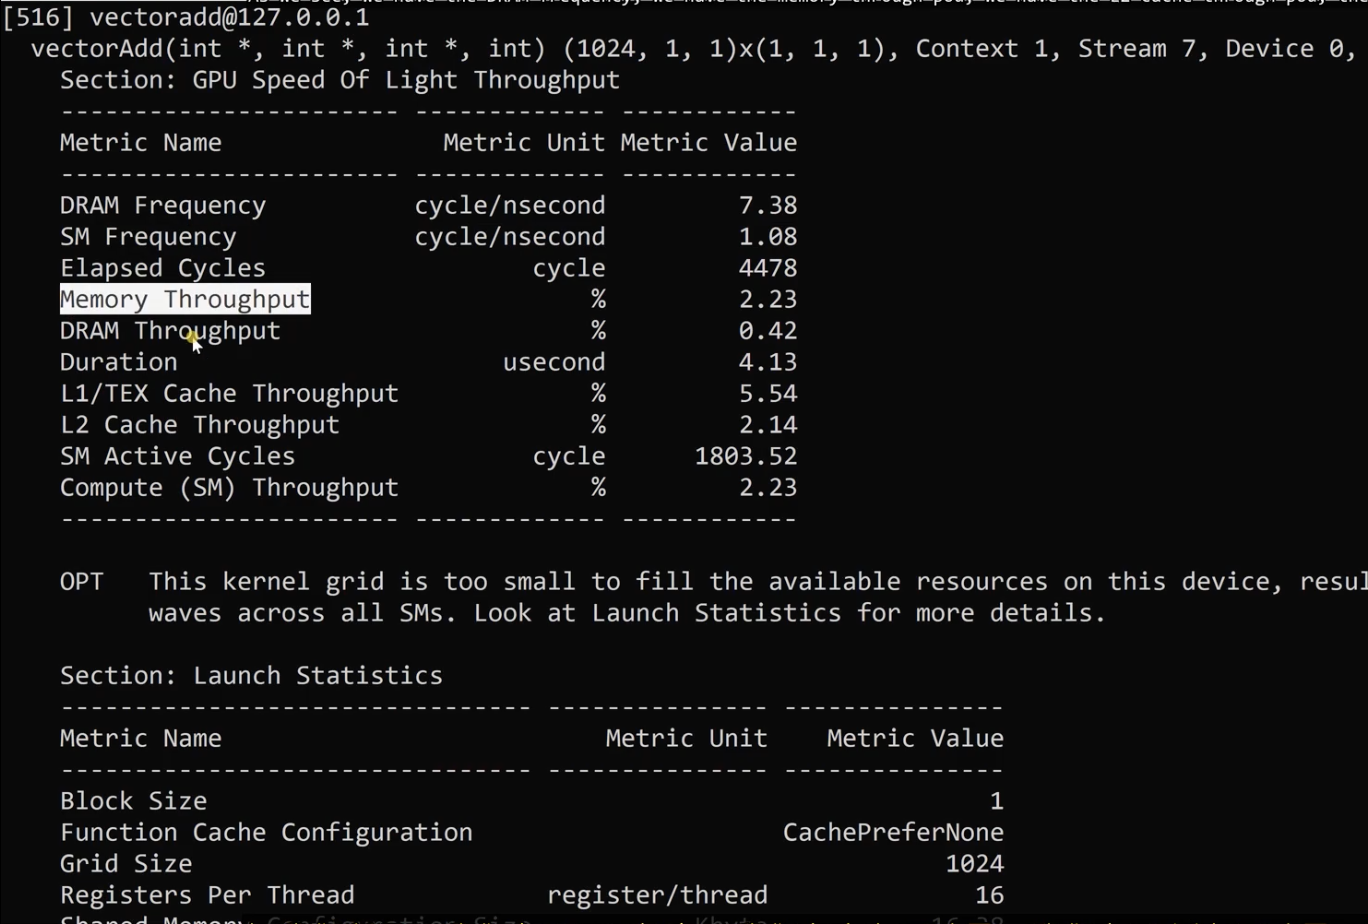
\includegraphics[width=0.75\linewidth]{resources/cuda-098.png}
    \caption{}
    \label{fig:placeholder}
\end{figure}


现在已经允许所有用户访问 GPU 性能计数器。回到这里，尝试使用命令。可以检查到错误中有一些变化。如所示，这些错误与之前的错误不同了。为了验证这一点，检查第一个错误，这里提到驱动程序，但现在这里不是关于驱动程序的。

接下来需要重启 Ubuntu 系统。输入 \texttt{sudo reboot}，然后点击回车。如果在使用 WSL（即在 Windows 上安装 Ubuntu 系统或 Linux 系统的工具），需要耐心一点。需要等待大约一分钟，然后再启动 Ubuntu 系统。等待超过一分钟后，通过输入 \texttt{wsl} 再次启动 Ubuntu 系统。等待几秒钟，然后进入文件夹。

输入 \texttt{cd cuda\_course}，然后再次运行相同的命令。如所示，得到了一些结果。有 DRAM 频率、内存吞吐量、L2 缓存吞吐量、活动周期，这些是 \texttt{ncu} 命令提供的度量指标。这里有一些配置，如块大小、网格大小，每个线程的寄存器数。还有一个名为占用率的部分，与前文讨论的占用率相关，这里有一些限制。最后有这个度量指标，即达到的占用率。本章不会解释这些度量指标，因为本章只是为了解决在 Windows 系统上运行 \texttt{ncu} 或 Nsight Compute 的问题。
